\documentclass[UTF8]{ctexart}
\usepackage{fullpage}
\usepackage{times}
\usepackage[normalem]{ulem}
\usepackage{multirow}
\usepackage{fancyhdr,graphicx,amsmath,amssymb, mathtools, scrextend, titlesec, enumitem}\usepackage[pdftex]{hyperref}
\usepackage[ruled,vlined]{algorithm2e}
\usepackage{parskip}
\usepackage{listings}
\usepackage{amsmath}
\usepackage{physics}
\usepackage{bbm}
\usepackage{titling}
\usepackage{bm}
\usepackage{geometry}
\geometry{top=1cm, left=1cm, bottom=1.5cm, right=1.5cm, margin=1cm}
\newcommand{\varvec}[2][n]{#2_1,\ldots, #2_#1}
\newcommand{\Var}{\mathrm{Var}}
\newcommand{\Bias}{\mathrm{Bias}}
\newcommand{\Cov}{\mathrm{Cov}}
\newcommand{\E}{{\rm I\kern-.3em E}}
\newcommand{\Binomial}{\mathrm{Binomial}}
\newcommand{\Bernoulli}{\mathrm{Bernoulli}}
\newcommand{\Poisson}{\mathrm{Poisson}}
\newcommand{\Normal}{\mathcal{N}}
\newcommand{\one}{\mathbbm{1}}
\newcommand{\Beta}{\text{Beta}}
\newcommand{\BetaPDF}{\text{Beta}}
\newcommand{\GammaPDF}{\text{Gamma}}
\newcommand{\Uniform}{\mathrm{Uniform}}
\newcommand{\QED}{\newline \mbox{} \hfill $\blacksquare$}
\newcommand{\Real}{\mathbb{R}}
\newcommand{\Sgn}{\mbox{Sgn}}
\renewcommand*{\arraystretch}{1.4}
\newtheorem{theorem}{Result}
\newtheorem{definition}{Definition}
\lstset{frame=tb,
	language=Python,
	aboveskip=3mm,
	belowskip=3mm,
	showstringspaces=false,
	columns=flexible,
	basicstyle={\small\ttfamily},
	numbers=none,
	stringstyle=\color{mauve},
	breaklines=true,
	breakatwhitespace=true,
	tabsize=3
}
\graphicspath{ {./imgs} }

\title{NURB}
\begin{document}
	\maketitle
\section{Bernstein Polynomial}

\textbf{Bernstein basis polynomial} of degree $n$ are 
$$ B_{i,n}(t) = \binom{n}{i} t^i (1 - t)^{n-i} \qquad ,(t \in \left[0, 1\right], \quad i = 1,\ldots,n)$$

\textbf{Bernstein polynomial} of degree $n$ is 
$$B_n(t) = \sum_{i=0}^{n} \beta_i B_{i, n}(t)$$
where $\beta_i$ is called Bernstein or Bezier coefficient.
	
Bernstein polynomial can approximate any continuous function on $\left[0, 1\right]$. 

$$ B_n(f)(t) = \sum_{i=0}^{n} f\left(\frac{i}{n}\right) B_{i, n}(t)$$
and  $$ \lim_{n\rightarrow \infty} B_n(f)(t) \xrightarrow{\text{uniformly}} f(t)$$


\section{Bezier Curve}

\begin{center}
	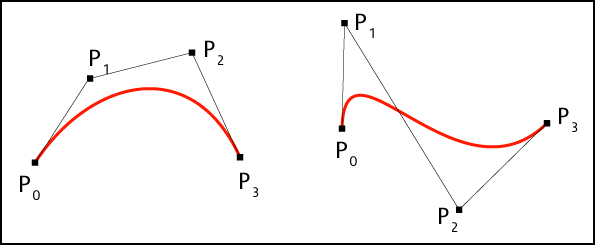
\includegraphics[scale=0.5]{bezier_01.jpg}
\end{center}

Given $n+1$ control points, $\boldsymbol{P}_1, \ldots, \boldsymbol{P}_n$,  a bezier curve is defined by 

$$ C(t) = \sum_{i=0}^{n} \boldsymbol{P}_i B_{i, n}(t)$$

$C(t)$ always passes through the first and the last control point and its tangent at $C(t_0)$ and $C(t_n)$ are $\overrightarrow{P_0P_1}$ and $\overrightarrow{P_{n-1}P_n}$ respectively.

\begin{center}
	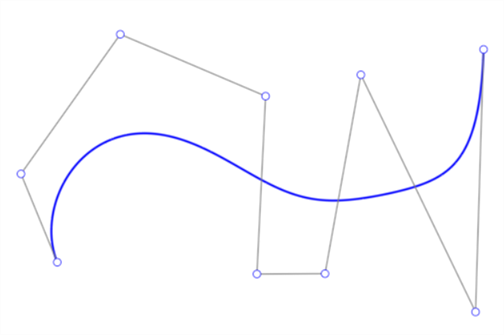
\includegraphics{bezier_02.png}
	\captionof{figure}{Bezier curve with more control points}
\end{center}

\section{B-Spline}
B-Spline is a generalization of Bezier curve. Given a knot vector $$T=\{t_0, \ldots, t_m  \quad|\quad t_i \in \left[0, 1\right], t_i \leq t_{i+1}\}$$

We can build B-Spline basis $N_{i, j}$ by bottom up recursion defined by 
\begin{Large}
$$
\begin{aligned}
&N_{i, 0}(t) = \begin{cases}
	I_{\left[t_i, t_{i+1}\right]}(t) &\quad\text{, if } t_i \neq t_{i+1} \\
	0 &\quad\text{, otherwise}
\end{cases} \\
&N_{i, j}(t) = \frac{t - t_i}{t_{i+j} - t_{i}} N_{i, j-1}(t) + \frac{t_{i+j+1} - t}{t_{i+j+1} - t_{i+1}} N_{i+1, j-1}(t)
\end{aligned}
$$

\begin{tcolorbox}[colback=white,colframe=cyan,width=\dimexpr\textwidth+12mm\relax,enlarge left by=-6mm]
For example, if $T=\{0, 1, 2, 3\}$, we can build the basis from bottom up recursively
\begin{center}
\begin{tikzpicture}
	\node[state] (n00) {$N_{0, 0}$};
	\node[state, right of=n00, xshift=2cm] (n10) {$N_{1, 0}$};
	\node[state, right of=n10, xshift=2cm] (n20) {$N_{2, 0}$};
	\node[state, below right of= n00, xshift=1cm, yshift=-2cm] (n01) {$N_{0, 1}$};
	\node[state, right of=n01, xshift=2cm] (n11) {$N_{1, 1}$};
	\node[state, below right of= n01, xshift=1cm, yshift=-2cm] (n02) {$N_{0, 2}$};
	\draw[-{Stealth[scale=1.5]}, thick] (n00) edge (n01);
	\draw[-{Stealth[scale=1.5]}, thick] (n10) edge (n01);
	\draw[-{Stealth[scale=1.5]}, thick] (n10) edge (n11);
	\draw[-{Stealth[scale=1.5]}, thick] (n20) edge (n11);
	\draw[-{Stealth[scale=1.5]}, thick] (n01) edge (n02);
	\draw[-{Stealth[scale=1.5]}, thick] (n11) edge (n02);
\end{tikzpicture}
\end{center}

We ended up with 
$$
 \begin{aligned}
 	&N_{0, 1} =  t I_{\left[0, 1\right]} + (2 - t) I_{\left[1, 2\right]} \\ 
 	&N_{1, 1} =  (t - 1) I_{\left[1, 2\right]} + (3 - t) I_{\left[2, 3\right]} \\
 	&N_{0, 2} = \frac{t^2}{2} I_{\left[0, 1\right]} + \frac{(6t - 2t^2 -3)}{2} I_{\left[1, 2\right]} + \frac{(3 - t)^2}{2}  I_{\left[2, 3\right]}
 \end{aligned}
$$

\end{tcolorbox}

With control points $C_0, \ldots, C_n$, we can define the degree of B-spline $D = m - n - 1$. And the B-spline is defined by the basis as 

$$ C(t) = \sum_{i = 0}^{D} C_i N_{i, D}(t) $$

Often times, control points are not given, instead we need to fit a B-spline to points $(P_0, t_0), \ldots , (P_m, t_m)$. Instead we solve for $C_i$, 

$$ P_i = C(t_i) = \sum_{j = 0}^{D} C_j N_{j, D}(t_i) \quad  \Rightarrow  \quad P = C N $$

\end{Large}
\end{document}